\section{Instalación}

Antes de empezar se tiene entendido que ya contamos con \textbf{python} y \textbf{pip} instalado en nuestra computadora. Los pasos a seguir están descritos en la documentación oficial de \href{https://www.djangoproject.com/}{\underline{Django}}. Un pre-paso antes de hacer la instalación es que deberán descargar el repositorio del proyecto, una vez descargado cambiar a la carpeta del proyecto.

\subsection{Django}

\subsubsection*{Linux}

El comando que nos da la documentación: \texttt{python -m pip install Django==5.0.3}, sin embargo es posible que tengan instalado \textit{python3}, en este caso bastará con hacer la siguiente modificación: 
\begin{center}
    \texttt{python3 -m pip install Django==5.0.3}    
\end{center}
Lo que estamos instalando es la versión más reciente de Django para ver la información podemos usar \texttt{pip show django} y para corroborar la instalación: \texttt{python3 -m django --version}

\begin{center}
    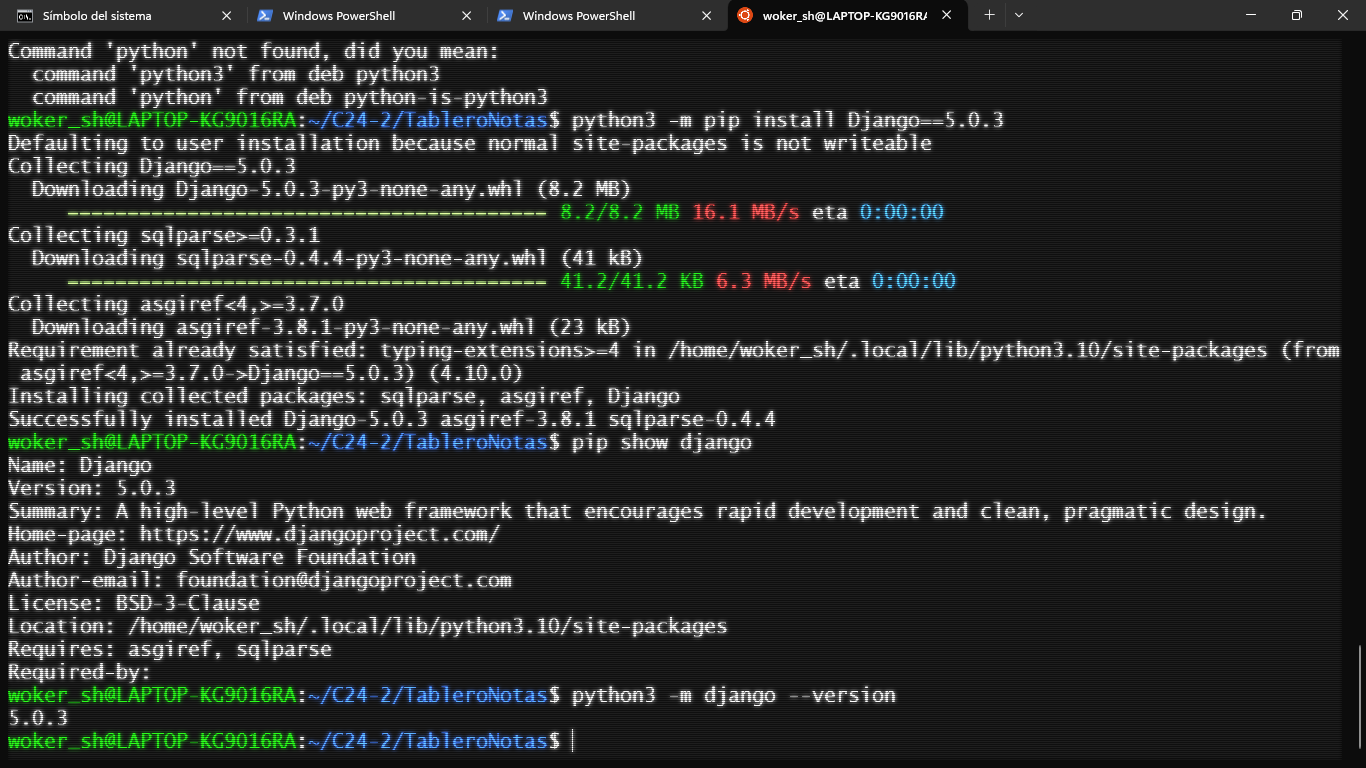
\includegraphics[scale = .35]{IMA/djangoLinux.png}
\end{center}

\subsubsection*{Windows}

El comando que nos da la documentación: \texttt{py -m django --version}. Al ejecutarlo posiblemente les pida actualizar \texttt{pip}. A pesar de hacer correcta la instalación con solo este comando tuve problemas al ejecutar el servidor de Django, al usar \texttt{show django} me decía que no se había instalado correctamente.

\begin{center}
    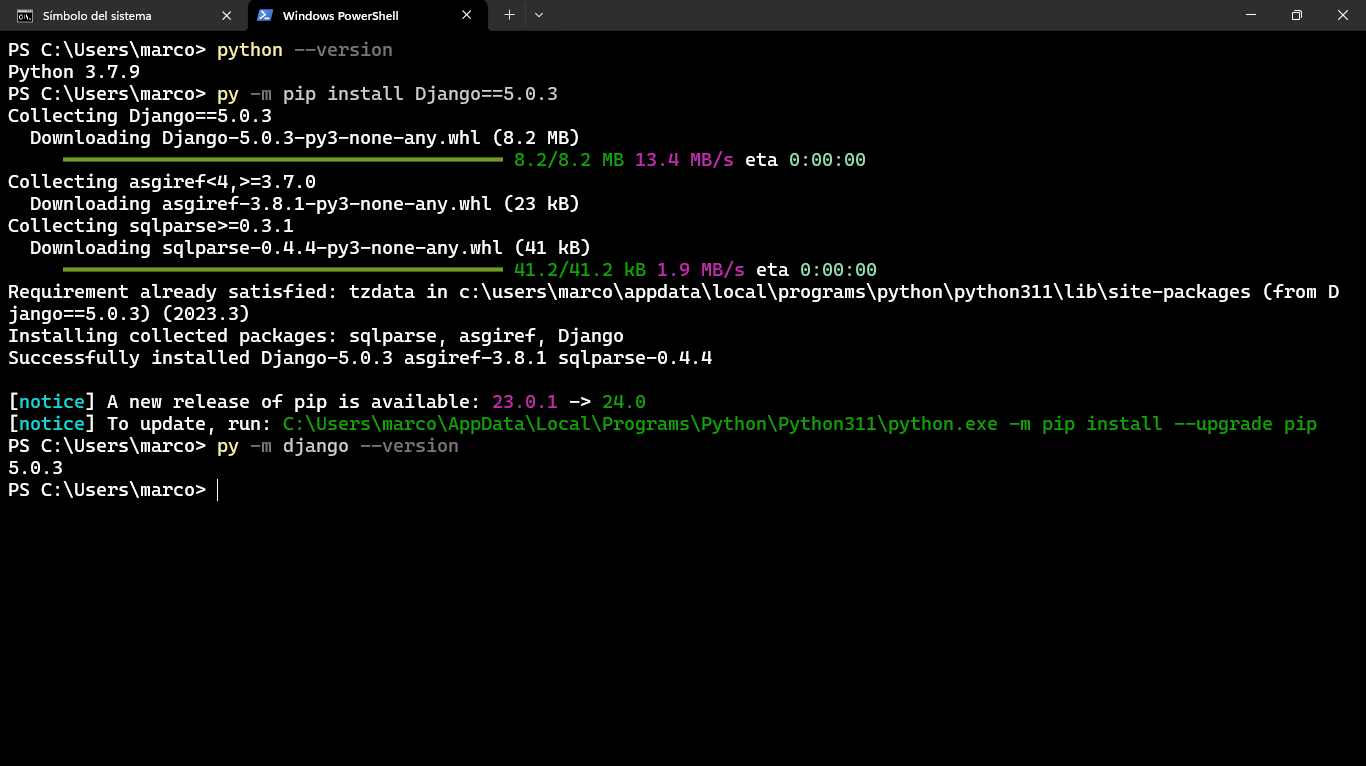
\includegraphics[scale = .35]{IMA/djangoWindo01.png}
\end{center}


Tuve que usar también este comando: \texttt{pip install django}

\begin{center}
    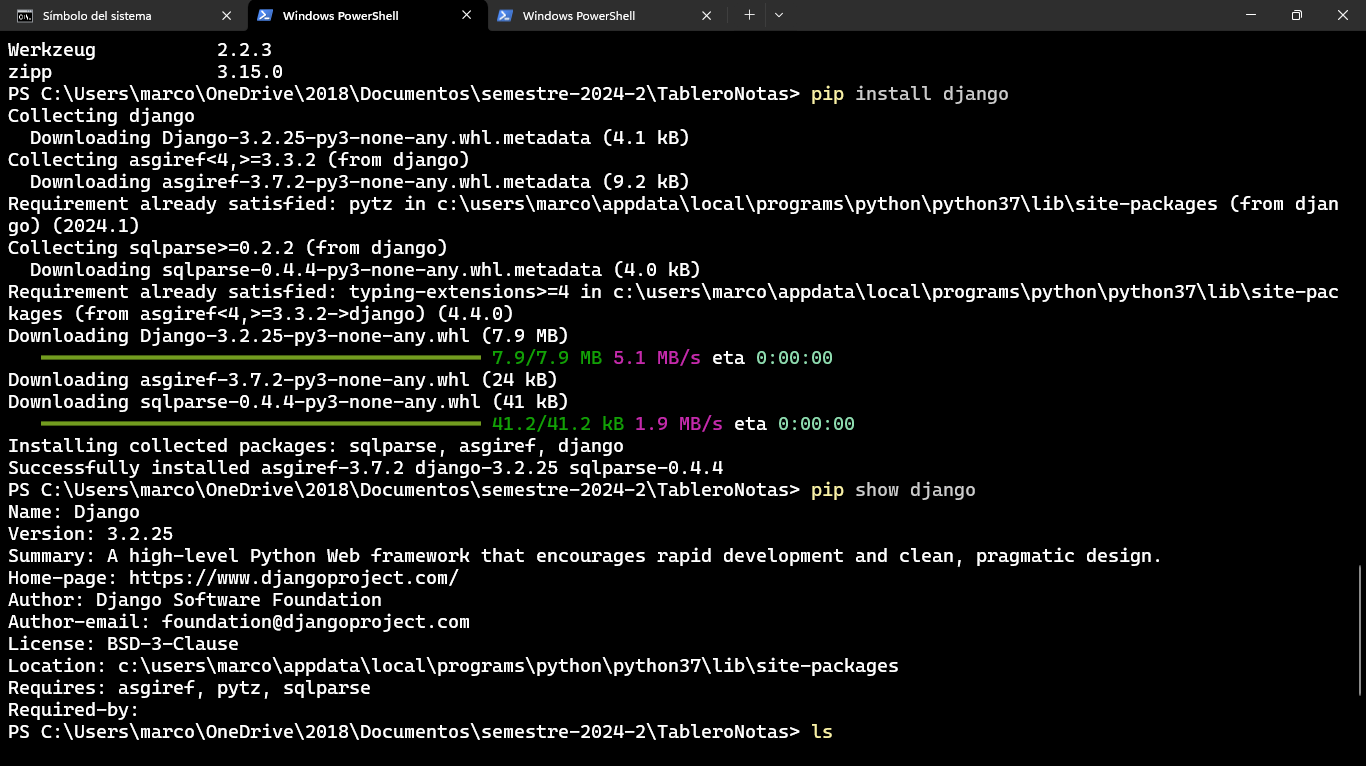
\includegraphics[scale = .47]{IMA/djangoWindo02.png}
\end{center}

Con esto ya se pudo ejecutar el servidor correctamente, para ambos distribuciones, recordad que se debe hacer dentro de la carpeta del proyecto.

\newpage
\section{Ejecución}

Para ejecutar el servidor y lo puedan ver dentro de su navegador

\begin{itemize}
    \item Windows:  \texttt{py manage.py runserver}    
    \item Linux: \texttt{python3 manage.py runserver}
\end{itemize}

Una vez iniciado el servidor, en el navegador debemos ir al puerto: \texttt{http://127.0.0.1:8000/}\\

Para salir del servidor usar \texttt{Ctrl + c}

\begin{center}
    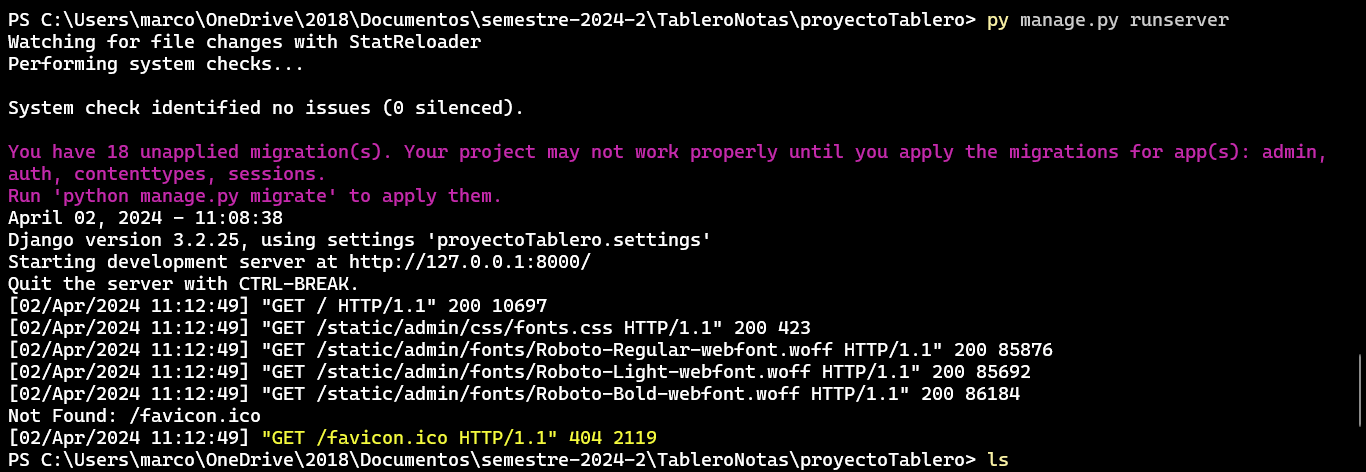
\includegraphics[scale = .47]{IMA/ejecucion.png}
\end{center}